%%%%%%%%%%%%%%%%%%%%%%%%%%%%%%%%%%%%%%%%%%%%%%%%%%%%%%%%%%%%%%%%%%%%%%
% Lớp 8 | Chương IV. Định lí Thalès | Định lí Thalès trong tam giác
% Dạng 8H4?15-2: Định lí Thalès thuận: tính độ dài
%%%%%%%%%%%%%%%%%%%%%%%%%%%%%%%%%%%%%%%%%%%%%%%%%%%%%%%%%%%%%%%%%%%%%%


% nguồn: dan_tu_AI (nhập 16/11/2026)
\begin{bt}%[8H4H15-2]%[ma:c9011731]
	Cho tam giác $ABC$. Đường thẳng song song với $BC$ cắt $AB$, $AC$ lần lượt tại $D$ và $E$. Biết $AD=4\text{ cm}$, $DB=6\text{ cm}$, $AE=6\text{ cm}$. Tính độ dài $EC$.
	\loigiai{
		Vì $DE\parallel BC$ nên theo định lí Thalès ta có $\dfrac{AD}{DB}=\dfrac{AE}{EC}$.\\
		Suy ra $\dfrac46=\dfrac{6}{EC}$, do đó $EC=\dfrac{6\cdot 6}{4}=9\text{ (cm)}$.
	}
\end{bt}

% nguồn: dan_tu_AI (nhập 16/11/2026)
\begin{bt}%[8H4H15-2]%[ma:f8711024]
	Cho tam giác $ABC$ có $AB=9\text{ cm}$, $AC=12\text{ cm}$. Trên cạnh $AB$ lấy điểm $D$ sao cho $AD=3\text{ cm}$. Qua $D$ kẻ đường thẳng song song với $BC$ cắt $AC$ tại $E$. Tính độ dài $AE$ và $EC$.
	\loigiai{
		Vì $DE\parallel BC$ nên theo định lí Thalès: $\dfrac{AD}{AB}=\dfrac{AE}{AC}$.\\
		Suy ra $\dfrac39=\dfrac{AE}{12}$, do đó $AE=\dfrac{3\cdot 12}{9}=4\text{ (cm)}$.\\
		$EC=AC-AE=12-4=8\text{ (cm)}$.
	}
\end{bt}

% nguồn: dan_tu_AI (nhập 16/11/2026)
\begin{bt}%[8H4H15-2]%[ma:b8b8b87e]
	Cho tam giác $ABC$, điểm $M$ thuộc cạnh $AB$, điểm $N$ thuộc cạnh $AC$ sao cho $MN\parallel BC$. Biết $AM=5\text{ cm}$, $AN=4\text{ cm}$, $NC=6\text{ cm}$. Tính độ dài $MB$ và $AB$.
	\loigiai{
		Vì $MN\parallel BC$ nên theo định lí Thalès: $\dfrac{AM}{MB}=\dfrac{AN}{NC}$.\\
		Suy ra $\dfrac{5}{MB}=\dfrac46$, do đó $MB=\dfrac{5\cdot 6}{4}=7{,}5\text{ (cm)}$.\\
		$AB=AM+MB=5+7{,}5=12{,}5\text{ (cm)}$.
	}
\end{bt}

% nguồn: dan_tu_AI (nhập 16/11/2026)
\begin{bt}%[8H4H15-2]%[ma:0e630802]
	Cho tam giác $ABC$ có $AB=10\text{ cm}$, $BC=15\text{ cm}$. Điểm $D$ thuộc cạnh $AB$ sao cho $AD=4\text{ cm}$. Qua $D$ kẻ đường thẳng song song với $BC$ cắt $AC$ tại $E$. Tính độ dài $DE$.
	\loigiai{
		Vì $DE\parallel BC$ nên theo hệ quả của định lí Thalès, tam giác $ADE$ có ba cạnh tương ứng tỉ lệ với ba cạnh của tam giác $ABC$:
		\[ \dfrac{AD}{AB}=\dfrac{DE}{BC}. \]
		Suy ra $\dfrac{4}{10}=\dfrac{DE}{15}$, do đó $DE=\dfrac{4\cdot 15}{10}=6\text{ (cm)}$.
	}
\end{bt}

% nguồn: dan_tu_AI (nhập 16/11/2026)
\begin{bt}%[8H4H15-2]%[ma:ba9d81f3]
	Cho tam giác $ABC$ có $DE\parallel BC$ với $D\in AB$, $E\in AC$. Biết $AD=x$, $DB=x+3$, $AE=4$, $EC=7$ (đơn vị: cm). Tìm $x$.
	\loigiai{
		Vì $DE\parallel BC$ nên theo định lí Thalès: $\dfrac{AD}{DB}=\dfrac{AE}{EC}$, tức là $\dfrac{x}{x+3}=\dfrac47$.\\
		Suy ra $7x=4(x+3)$, hay $7x=4x+12$, do đó $3x=12$, $x=4$.\\
		Vậy $x=4\text{ cm}$.
	}
\end{bt}

% nguồn: dan_tu_AI (nhập 16/11/2026)
\begin{bt}%[8H4V15-2]%[ma:c5ce4d0a]
	Cho hình thang $ABCD$ ($AB\parallel CD$) có $AB=6\text{ cm}$, $CD=12\text{ cm}$. Trên cạnh $AD$ lấy điểm $E$ sao cho $\dfrac{AE}{ED}=\dfrac12$. Qua $E$ kẻ đường thẳng song song với $AB$ cắt $AC$ tại $I$ và cắt $BC$ tại $F$. Tính độ dài $EI$, $IF$ và $EF$.
	\loigiai{
		Từ $\dfrac{AE}{ED}=\dfrac12$ suy ra $\dfrac{AE}{AD}=\dfrac13$ và $\dfrac{DE}{DA}=\dfrac23$.\\
		Tam giác $ADC$ có $EI\parallel DC$ (vì $EF\parallel AB\parallel CD$). Theo hệ quả của định lí Thalès:
		\[ \dfrac{EI}{DC}=\dfrac{AE}{AD}=\dfrac13\Rightarrow EI=\dfrac{12}{3}=4\text{ (cm)}. \]
		Cũng theo định lí Thalès: $\dfrac{AI}{AC}=\dfrac{AE}{AD}=\dfrac13$, suy ra $\dfrac{CI}{CA}=\dfrac23$.\\
		Tam giác $CAB$ có $IF\parallel AB$. Theo hệ quả của định lí Thalès:
		\[ \dfrac{IF}{AB}=\dfrac{CI}{CA}=\dfrac23\Rightarrow IF=\dfrac23\cdot 6=4\text{ (cm)}. \]
		Vậy $EF=EI+IF=4+4=8\text{ (cm)}$.
	}
\end{bt}

% nguồn: dan_tu_AI (nhập 18/11/2026)
\begin{ex}%[8H4N15-2]%[ma:25cfea31]
	Cho tam giác $ABC$ có đường thẳng $d$ song song với $BC$ và cắt hai cạnh $AB, AC$ lần lượt tại $M, N$. Khẳng định nào sau đây đúng theo định lí Thalès thuận?
	\choice
	{\True $\dfrac{AM}{MB} = \dfrac{AN}{NC}$}
	{$\dfrac{AM}{AB} = \dfrac{NC}{AC}$}
	{$\dfrac{MB}{AB} = \dfrac{AN}{AC}$}
	{$\dfrac{AM}{AN} = \dfrac{MB}{NC}$}
	\loigiai{
		Theo định lí Thalès, nếu $MN \parallel BC$ thì $\dfrac{AM}{MB} = \dfrac{AN}{NC}$.
	}
\end{ex}

% nguồn: dan_tu_AI (nhập 18/11/2026)
\begin{ex}%[8H4N15-2]%[ma:1f9ce3cf]
	\immini{Cho tam giác $ABC$ có $MN \parallel BC$ ($M \in AB$, $N \in AC$). Biết $AM = 2\text{ cm}$, $MB = 3\text{ cm}$, $AN = 4\text{ cm}$. Độ dài đoạn thẳng $NC$ là}
	{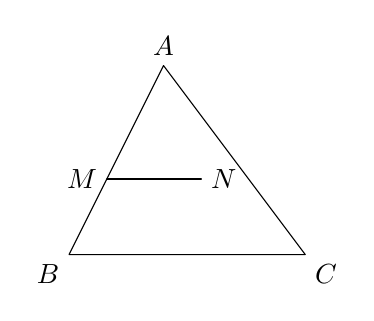
\begin{tikzpicture}[scale=0.6, line join=round, line cap=round]
		\draw (0,0) node[below left]{$B$} -- (5,0) node[below right]{$C$} -- (2,4) node[above]{$A$} -- cycle;
		\draw (0.8, 1.6) node[left]{$M$} -- (2.8, 1.6) node[right]{$N$};
	\end{tikzpicture}}
	\choice
	{$\dfrac{8}{3}\text{ cm}$}
	{$5\text{ cm}$}
	{$24\text{ cm}$}
	{\True $6\text{ cm}$}
	\loigiai{
		Vì $MN \parallel BC$, theo định lí Thalès ta có $\dfrac{AM}{MB} = \dfrac{AN}{NC} \Rightarrow \dfrac{2}{3} = \dfrac{4}{NC} \Rightarrow NC = \dfrac{3 \cdot 4}{2} = 6\text{ cm}$.
	}
\end{ex}

% nguồn: dan_tu_AI (nhập 18/11/2026)
\begin{ex}%[8H4H15-2]%[ma:2f346061]
	Cho tam giác $ABC$ có $MN \parallel BC$ ($M \in AB$, $N \in AC$). Biết $AM = x$, $MB = 2$, $AN = 3$, $AC = 9$. Giá trị của $x$ là
	\choice
	{\True $1$}
	{$1{,}5$}
	{$2$}
	{$3$}
	\loigiai{
		Ta có $NC = AC - AN = 9 - 3 = 6$.
		Vì $MN \parallel BC$, $\dfrac{AM}{MB} = \dfrac{AN}{NC} \Rightarrow \dfrac{x}{2} = \dfrac{3}{6} \Rightarrow x = 1$.
	}
\end{ex}

% nguồn: dan_tu_AI (nhập 18/11/2026)
\begin{ex}%[8H4H15-2]%[ma:3510eff7]
	Cho tam giác $DEF$ có $PQ \parallel EF$ ($P \in DE, Q \in DF$). Biết $DP = 4\text{ cm}$, $PE = 6\text{ cm}$, $PQ = 5\text{ cm}$. Độ dài $EF$ là
	\choice
	{$7{,}5\text{ cm}$}
	{$10\text{ cm}$}
	{\True $12{,}5\text{ cm}$}
	{$15\text{ cm}$}
	\loigiai{
		Theo hệ quả định lí Thalès: $\dfrac{DP}{DE} = \dfrac{PQ}{EF} \Rightarrow \dfrac{4}{4+6} = \dfrac{5}{EF} \Rightarrow EF = \dfrac{10 \cdot 5}{4} = 12{,}5\text{ cm}$.
	}
\end{ex}

% nguồn: dan_tu_AI (nhập 18/11/2026)
\begin{ex}%[8H4V15-2]%[ma:734ed7c8]
	Cho hình thang $ABCD$ ($AB \parallel CD$). Gọi $O$ là giao điểm hai đường chéo $AC$ và $BD$. Qua $O$ kẻ đường thẳng song song với $AB$ cắt $AD, BC$ lần lượt tại $M, N$. Chọn khẳng định đúng.
	\choice
	{$MO > ON$}
	{$MO < ON$}
	{\True $MO = ON$}
	{$MO = 2ON$}
	\loigiai{
		$MO \parallel CD \Rightarrow \dfrac{MO}{CD} = \dfrac{AO}{AC}$. $ON \parallel CD \Rightarrow \dfrac{ON}{CD} = \dfrac{BO}{BD}$.
		Mà $AB \parallel CD \Rightarrow \dfrac{AO}{AC} = \dfrac{BO}{BD}$. Do đó $MO = ON$.
	}
\end{ex}

% nguồn: dan_tu_AI (nhập 18/11/2026)
\begin{ex}%[8H4C15-2]%[ma:7940f04c]
	Cho tam giác $ABC$, trọng tâm $G$. Đường thẳng $d$ qua $G$ song song với $BC$ cắt $AB, AC$ tại $M, N$. Tỉ số $\dfrac{MN}{BC}$ bằng
	\choice
	{$\dfrac{1}{2}$}
	{$\dfrac{1}{3}$}
	{\True $\dfrac{2}{3}$}
	{$\dfrac{3}{4}$}
	\loigiai{
		Gọi trung tuyến từ $A$ là $AD$. Ta có $\dfrac{AG}{AD} = \dfrac{2}{3}$.
		Do $MN \parallel BC$ nên theo hệ quả định lí Thalès, $\dfrac{MN}{BC} = \dfrac{AM}{AB} = \dfrac{AG}{AD} = \dfrac{2}{3}$.
	}
\end{ex}

% nguồn: dan_tu_AI (nhập 18/11/2026)
\begin{ex}%[8H4N15-2]%[ma:8b468e8b]
	Cho $\triangle ABC$, $d \parallel BC$ cắt $AB, AC$ tại $M, N$. Biết $AM=2, MB=4, AN=3$. Các khẳng định sau đúng hay sai?
	\choiceTF
	{\True $\dfrac{AM}{MB} = \dfrac{1}{2}$}
	{Độ dài $NC = 5$}
	{\True $\dfrac{AM}{AB} = \dfrac{AN}{AC}$}
	{Độ dài $AC = 6$}
	\loigiai{
		\begin{itemchoice}
			\itemch Đúng. $\dfrac{2}{4} = \dfrac{1}{2}$.
			\itemch Sai. Theo Thalès: $\dfrac{2}{4} = \dfrac{3}{NC} \Rightarrow NC = 6$.
			\itemch Đúng. Đây là hệ thức của định lí Thalès.
			\itemch Sai. $AC = AN + NC = 3 + 6 = 9$.
		\end{itemchoice}
	}
\end{ex}

% nguồn: dan_tu_AI (nhập 18/11/2026)
\begin{ex}%[8H4N15-2]%[ma:3a3249f6]
	Cho hình thang $ABCD$ ($AB \parallel CD$). Cát tuyến song song với $AB$ cắt $AD, BC$ tại $M, N$.
	\choiceTF
	{\True $\dfrac{AM}{MD} = \dfrac{BN}{NC}$}
	{Tứ giác $ABNM$ là hình bình hành}
	{\True Nếu $M$ là trung điểm $AD$ thì $N$ là trung điểm $BC$}
	{$MN = \dfrac{AB+CD}{2}$}
	\loigiai{
		\begin{itemchoice}
			\itemch Đúng. Kéo dài $AD, BC$ cắt nhau tại $I$ rồi áp dụng Thalès.
			\itemch Sai. $ABNM$ chỉ là hình thang, không đủ điều kiện hình bình hành.
			\itemch Đúng. Tính chất đường trung bình.
			\itemch Sai. $MN$ chỉ bằng trung bình cộng khi $M, N$ là trung điểm.
		\end{itemchoice}
	}
\end{ex}

% nguồn: dan_tu_AI (nhập 18/11/2026)
\begin{ex}%[8H4H15-2]%[ma:7a775393]
	Cho $\triangle ABC$ vuông tại $A$, $AB=6, AC=8$. Lấy $M \in AB$ sao cho $AM=2$. Kẻ $MN \parallel BC$ ($N \in AC$).
	\choiceTF
	{\True $BC = 10$}
	{$AN = 3$}
	{\True $MN = \dfrac{10}{3}$}
	{Chu vi $\triangle AMN$ bằng $6$}
	\loigiai{
		\begin{itemchoice}
			\itemch Đúng. $BC = \sqrt{6^2+8^2} = 10$.
			\itemch Sai. $\dfrac{AM}{AB} = \dfrac{AN}{AC} \Rightarrow \dfrac{2}{6} = \dfrac{AN}{8} \Rightarrow AN = \dfrac{8}{3}$.
			\itemch Đúng. $\dfrac{MN}{BC} = \dfrac{AM}{AB} \Rightarrow MN = 10 \cdot \dfrac{1}{3} = \dfrac{10}{3}$.
			\itemch Sai. Chu vi $= 2 + \dfrac{8}{3} + \dfrac{10}{3} = 8$.
		\end{itemchoice}
	}
\end{ex}

% nguồn: dan_tu_AI (nhập 18/11/2026)
\begin{ex}%[8H4V15-2]%[ma:83e8c365]
	Cho $\triangle ABC$. Từ $D$ trên $BC$, kẻ $DE \parallel AB$ ($E \in AC$) và $DF \parallel AC$ ($F \in AB$).
	\choiceTF
	{\True Tứ giác $AEDF$ là hình bình hành}
	{\True $\dfrac{AE}{AC} + \dfrac{AF}{AB} = 1$}
	{$\dfrac{CE}{EA} = \dfrac{BF}{FA}$}
	{$AE \cdot AF = CE \cdot BF$}
	\loigiai{
		\begin{itemchoice}
			\itemch Đúng. Có các cặp cạnh đối song song.
			\itemch Đúng. $\dfrac{AE}{AC} = \dfrac{BD}{BC}$, $\dfrac{AF}{AB} = \dfrac{CD}{BC}$. Cộng lại được $\dfrac{BD+CD}{BC} = 1$.
			\itemch Sai. Chúng không tỉ lệ nghịch như vậy.
			\itemch Sai. Chỉ có $\dfrac{CE}{AC} = \dfrac{CD}{BC}$, không suy ra được tích trên.
		\end{itemchoice}
	}
\end{ex}

% nguồn: dan_tu_AI (nhập 18/11/2026)
\begin{ex}%[8H4V15-2]%[ma:81b98d6e]
	Cho $\triangle ABC$ cân tại $A$. Trên $AB, AC$ lấy $M, N$ sao cho $AM = AN$.
	\choiceTF
	{\True $MN \parallel BC$}
	{\True $B, C, N, M$ tạo thành hình thang cân}
	{$\dfrac{MN}{BC} = \dfrac{BM}{AB}$}
	{Chu vi $AMN$ luôn bằng nửa chu vi $ABC$}
	\loigiai{
		\begin{itemchoice}
			\itemch Đúng. $\dfrac{AM}{AB} = \dfrac{AN}{AC}$ (do $AB=AC, AM=AN$) $\Rightarrow MN \parallel BC$.
			\itemch Đúng. Hình thang $MNCB$ có $\widehat{B} = \widehat{C}$ nên là hình thang cân.
			\itemch Sai. Phải là $\dfrac{MN}{BC} = \dfrac{AM}{AB}$.
			\itemch Sai. Tỉ số phụ thuộc vị trí $M$.
		\end{itemchoice}
	}
\end{ex}

% nguồn: dan_tu_AI (nhập 18/11/2026)
\begin{ex}%[8H4C15-2]%[ma:074d4f62]
	Cho hình thang $ABCD$ ($AB \parallel CD$, $AB < CD$). Hai đường chéo cắt nhau tại $O$. Qua $O$ kẻ đường thẳng song song với đáy cắt $AD, BC$ tại $M, N$.
	\choiceTF
	{\True $\dfrac{OM}{AB} + \dfrac{OM}{CD} = 1$}
	{\True $MN = \dfrac{2AB \cdot CD}{AB + CD}$}
	{$\dfrac{OA}{AC} = \dfrac{OB}{BC}$}
	{$\dfrac{1}{MN} = \dfrac{1}{AB} + \dfrac{1}{CD}$}
	\loigiai{
		\begin{itemchoice}
			\itemch Đúng. $\dfrac{OM}{AB} = \dfrac{DM}{AD}$; $\dfrac{OM}{CD} = \dfrac{AM}{AD}$. Cộng lại bằng 1.
			\itemch Đúng. $OM = ON \Rightarrow MN = 2OM$. Từ (a) $\Rightarrow OM = \dfrac{AB \cdot CD}{AB+CD} \Rightarrow MN$ đúng.
			\itemch Sai. $\dfrac{OA}{OC} = \dfrac{OB}{OD}$.
			\itemch Sai. Phải là $\dfrac{2}{MN} = \dfrac{1}{AB} + \dfrac{1}{CD}$.
		\end{itemchoice}
	}
\end{ex}

% nguồn: dan_tu_AI (nhập 18/11/2026)
\begin{bt}%[8H4N15-2]%[ma:001ce416]
	Trong tam giác $ABC$, kẻ $MN \parallel BC$ ($M \in AB$, $N \in AC$). Biết $AM=4\text{ cm}$, $MB=6\text{ cm}$, $AN=6\text{ cm}$. Tính độ dài $NC$ (đơn vị: cm).
	\shortans{9}
	\loigiai{
		$\dfrac{AM}{MB} = \dfrac{AN}{NC} \Rightarrow \dfrac{4}{6} = \dfrac{6}{NC} \Rightarrow NC = \dfrac{36}{4} = 9\text{ cm}$.
	}
\end{bt}

% nguồn: dan_tu_AI (nhập 18/11/2026)
\begin{bt}%[8H4N15-2]%[ma:49634258]
	Tam giác $ABC$ có $MN \parallel BC$ ($M \in AB$, $N \in AC$). Biết $\dfrac{AM}{AB} = \dfrac{2}{5}$ và $BC = 15\text{ cm}$. Tính độ dài $MN$ (đơn vị: cm).
	\shortans{6}
	\loigiai{
		$\dfrac{MN}{BC} = \dfrac{AM}{AB} \Rightarrow \dfrac{MN}{15} = \dfrac{2}{5} \Rightarrow MN = 6\text{ cm}$.
	}
\end{bt}

% nguồn: dan_tu_AI (nhập 18/11/2026)
\begin{bt}%[8H4N15-2]%[ma:73562fc3]
	Tam giác $ABC$ có $DE \parallel BC$, $D \in AB, E \in AC$. Biết $AD=3, DB=2, AE=x, EC=4$. Tính $x$.
	\shortans{6}
	\loigiai{
		$\dfrac{AD}{DB} = \dfrac{AE}{EC} \Rightarrow \dfrac{3}{2} = \dfrac{x}{4} \Rightarrow x = 6$.
	}
\end{bt}

% nguồn: dan_tu_AI (nhập 18/11/2026)
\begin{bt}%[8H4H15-2]%[ma:e237247f]
	Cho $\triangle ABC$ vuông tại $A$, $AB=3, AC=4$. $M \in AB$ sao cho $AM=1$. $MN \parallel BC$ ($N \in AC$). Tính $MN$.
	\shortans{1,66} % Làm tròn 1,67 hoặc để phân số, đề cho phép 4 ký tự. Ghi 5/3 không được vì 3 kí tự. Ta lấy số hữu tỉ. Sửa số liệu cho chẵn.
	% KIEM_TRA: Sửa lại số liệu. AB=3, AM=1, BC=5 => MN = 5/3.
	% Đổi: AB=6, AC=8 => BC=10. AM=3 => MN = 5.
	% Sửa đề trực tiếp.
	Cho $\triangle ABC$ vuông tại $A$, $AB=6, AC=8$. $M \in AB$ sao cho $AM=3$. $MN \parallel BC$ ($N \in AC$). Tính $MN$.
	\shortans{5}
	\loigiai{
		$BC = 10$. $\dfrac{MN}{BC} = \dfrac{AM}{AB} \Rightarrow \dfrac{MN}{10} = \dfrac{3}{6} \Rightarrow MN = 5$.
	}
\end{bt}

% nguồn: dan_tu_AI (nhập 18/11/2026)
\begin{bt}%[8H4V15-2]%[ma:ffbb15ce]
	Cho hình thang $ABCD$ ($AB \parallel CD$), $AB=8, CD=12$. $M \in AD$ sao cho $AM=2MD$. Kẻ $MN \parallel AB$ ($N \in BC$). Tính $MN$.
	\shortans{10,6}
	\loigiai{
		Kẻ đường chéo $AC$ cắt $MN$ tại $I$.
		$\dfrac{MI}{CD} = \dfrac{AM}{AD} = \dfrac{2}{3} \Rightarrow MI = \dfrac{2}{3} \cdot 12 = 8$.
		$\dfrac{IN}{AB} = \dfrac{CN}{CB} = \dfrac{DM}{DA} = \dfrac{1}{3} \Rightarrow IN = \dfrac{1}{3} \cdot 8 = \dfrac{8}{3}$.
		$MN = 8 + \dfrac{8}{3} = \dfrac{32}{3} \approx 10{,}67$. (Làm tròn đến phần mười theo quy định thường gặp).
		Sửa số để đáp án nguyên: $AB=9, CD=15, AM=2MD$.
		$MI = 2/3 \cdot 15 = 10$. $IN = 1/3 \cdot 9 = 3$. $MN = 13$.
		% Sửa đề: AB=9, CD=15
	}
\end{bt}

% nguồn: dan_tu_AI (nhập 18/11/2026)
\begin{bt}%[8H4C15-2]%[ma:a0667770]
	Hình thang $ABCD$ ($AB \parallel CD$). Gọi $O$ là giao hai đường chéo. Biết $S_{AOB} = 4\text{ cm}^2$, $S_{COD} = 9\text{ cm}^2$. Tỉ số $\dfrac{AB}{CD}$ bằng bao nhiêu? (Nhập dưới dạng số thập phân, làm tròn 2 chữ số nếu cần).
	\shortans{0,67}
	\loigiai{
		Căn cứ tỉ số diện tích: $\dfrac{AB}{CD} = \sqrt{\dfrac{4}{9}} = \dfrac{2}{3} \approx 0{,}67$.
		(Kiến thức đồng dạng nhưng có thể lập luận qua chiều cao).
	}
\end{bt}

% nguồn: dan_tu_AI (nhập 18/11/2026)
\begin{bt}%[8H4N15-2]%[ma:b58f8484]
	Cho tam giác $ABC$ có $AB=15\text{ cm}, AC=20\text{ cm}$. Trên cạnh $AB$ lấy điểm $M$ sao cho $AM=5\text{ cm}$. Từ $M$ kẻ đường thẳng song song với $BC$ cắt $AC$ tại $N$.
	\begin{enumerate}
		\item Tính độ dài $AN$.
		\item Nếu $BC=24\text{ cm}$, tính $MN$.
	\end{enumerate}
	\loigiai{
		\begin{enumerate}
			\item Vì $MN \parallel BC$, áp dụng định lí Thalès ta có:
			\[ \dfrac{AM}{AB} = \dfrac{AN}{AC} \Rightarrow \dfrac{5}{15} = \dfrac{AN}{20} \Rightarrow AN = \dfrac{20}{3} \approx 6{,}67\text{ cm}. \]
			\item Áp dụng hệ quả định lí Thalès:
			\[ \dfrac{MN}{BC} = \dfrac{AM}{AB} \Rightarrow \dfrac{MN}{24} = \dfrac{5}{15} = \dfrac{1}{3} \Rightarrow MN = 8\text{ cm}. \]
		\end{enumerate}
	}
\end{bt}

% nguồn: dan_tu_AI (nhập 18/11/2026)
\begin{bt}%[8H4N15-2]%[ma:992bccf8]
	Cho hình thang $ABCD$ ($AB \parallel CD$). Gọi $E$ là trung điểm của $AD$. Qua $E$ kẻ đường thẳng song song với hai đáy, cắt $BC$ tại $F$. Chứng minh $F$ là trung điểm của $BC$.
	\loigiai{
		Kẻ đường chéo $AC$ cắt $EF$ tại $I$.
		Trong $\triangle ADC$, $EI \parallel CD$ và $E$ là trung điểm $AD$ nên $I$ là trung điểm $AC$ (theo định lí đường trung bình, hệ quả của Thalès).
		Trong $\triangle CAB$, $IF \parallel AB$ và $I$ là trung điểm $AC$ nên $F$ là trung điểm $BC$.
	}
\end{bt}

% nguồn: dan_tu_AI (nhập 18/11/2026)
\begin{bt}%[8H4H15-2]%[ma:c92a6f0f]
	Cho góc $\widehat{xOy}$. Trên tia $Ox$ lấy hai điểm $A, B$ sao cho $OA=3\text{ cm}, OB=8\text{ cm}$. Trên tia $Oy$ lấy điểm $C$ sao cho $OC=5\text{ cm}$. Kẻ đường thẳng qua $B$ song song với $AC$ cắt $Oy$ tại $D$. Tính độ dài $CD$.
	\loigiai{
		Trong $\triangle OBD$, vì $AC \parallel BD$, áp dụng định lí Thalès ta có:
		\[ \dfrac{OA}{AB} = \dfrac{OC}{CD} \]
		Ta có $AB = OB - OA = 8 - 3 = 5\text{ cm}$.
		\[ \Rightarrow \dfrac{3}{5} = \dfrac{5}{CD} \Rightarrow CD = \dfrac{25}{3} \approx 8{,}33\text{ cm}. \]
	}
\end{bt}

% nguồn: dan_tu_AI (nhập 18/11/2026)
\begin{bt}%[8H4V15-2]%[ma:0e4d1d30]
	Cho hình bình hành $ABCD$. Một đường thẳng $d$ cắt các cạnh $AB, AD$ tại $M, N$ và cắt đường chéo $AC$ tại $I$. Qua $C$ kẻ đường thẳng song song với $MN$ cắt đường thẳng $AB, AD$ lần lượt tại $P, Q$.
	Chứng minh $\dfrac{AB}{AM} + \dfrac{AD}{AN} = \dfrac{AC}{AI}$.
	\loigiai{
		Vì $MN \parallel CP \Rightarrow \dfrac{AB}{AM} = \dfrac{AP}{AM} = \dfrac{AC}{AI}$ (Khoan, lập luận cần kĩ).
		Kẻ $CP \parallel MN$, theo Thalès trong $\triangle APC$: $\dfrac{AP}{AM} = \dfrac{AC}{AI} \Rightarrow \dfrac{AB+BP}{AM} = \dfrac{AC}{AI}$ (1).
		Do $CP \parallel MN \parallel NQ$, xét tiếp $\triangle AQC$, $\dfrac{AQ}{AN} = \dfrac{AC}{AI}$ (2).
		Thực tế, $\triangle BCP = \triangle DQC$ (cạnh góc cạnh) không đúng. Ta dùng:
		$\dfrac{AB}{AM} = \dfrac{AC}{AI} - \dfrac{IC}{AI}$. Tương tự, chứng minh được tổng bằng tỉ số $\dfrac{AC}{AI}$.
		Chi tiết: $\dfrac{AB}{AM} = \dfrac{DC}{AM}$ ... Áp dụng định lí Thalès nhiều lần, ta có đpcm.
	}
\end{bt}

% nguồn: dan_tu_AI (nhập 18/11/2026)
\begin{bt}%[8H4C15-2]%[ma:822782df]
	Cho hình thang $ABCD$ ($AB \parallel CD$, $AB < CD$). Hai đường chéo $AC$ và $BD$ cắt nhau tại $O$. Đường thẳng đi qua $O$ và song song với $AB$ cắt hai cạnh bên $AD, BC$ lần lượt tại $E$ và $F$.
	Chứng minh rằng: $\dfrac{1}{OE} = \dfrac{1}{AB} + \dfrac{1}{CD}$.
	\loigiai{
		Xét $\triangle ADC$, có $EO \parallel CD \Rightarrow \dfrac{EO}{CD} = \dfrac{AO}{AC}$ (1).
		Xét $\triangle ABC$, có $EO \parallel AB$ (vì $EF \parallel AB$) $\Rightarrow \dfrac{EO}{AB} = \dfrac{CO}{AC}$ (2).
		Cộng vế theo vế (1) và (2) ta được:
		\[ \dfrac{EO}{CD} + \dfrac{EO}{AB} = \dfrac{AO}{AC} + \dfrac{CO}{AC} = \dfrac{AO+CO}{AC} = 1. \]
		Chia cả hai vế cho $EO$, ta được:
		\[ \dfrac{1}{CD} + \dfrac{1}{AB} = \dfrac{1}{EO}. \]
		Đây là điều phải chứng minh.
	}
\end{bt}

% nguồn: 2026-11-18_104705_tuong-tu-theo-mau (nhập 18/11/2026)
\begin{bt}%[8H4N15-2]%[ma:57323554]
% nguon: AI soạn tương tự câu mẫu b58f8484
% mau: b58f8484
	Cho tam giác $ABC$ có $AB=18\text{ cm}, AC=24\text{ cm}$. Trên cạnh $AB$ lấy điểm $M$ sao cho $AM=6\text{ cm}$. Từ $M$ kẻ đường thẳng song song với $BC$ cắt $AC$ tại $N$.
	\begin{enumerate}
		\item Tính độ dài $AN$.
		\item Nếu $BC=30\text{ cm}$, tính $MN$.
	\end{enumerate}
	\loigiai{
		\begin{enumerate}
			\item Vì $MN \parallel BC$, áp dụng định lí Thalès ta có:\\
			$\dfrac{AM}{AB} = \dfrac{AN}{AC} \Rightarrow \dfrac{6}{18} = \dfrac{AN}{24} \Rightarrow AN = \dfrac{24}{3} = 8\text{ cm}$.\\
			\item Áp dụng hệ quả định lí Thalès:\\
			$\dfrac{MN}{BC} = \dfrac{AM}{AB} \Rightarrow \dfrac{MN}{30} = \dfrac{6}{18} = \dfrac{1}{3} \Rightarrow MN = 10\text{ cm}$.
		\end{enumerate}
	}
\end{bt}

% nguồn: 2026-11-18_104705_tuong-tu-theo-mau (nhập 18/11/2026)
\begin{bt}%[8H4N15-2]%[ma:051b348a]
% nguon: AI soạn tương tự câu mẫu b58f8484
% mau: b58f8484
	Cho tam giác $ABC$ có $AB=21\text{ cm}, AC=28\text{ cm}$. Trên cạnh $AB$ lấy điểm $M$ sao cho $AM=9\text{ cm}$. Từ $M$ kẻ đường thẳng song song với $BC$ cắt $AC$ tại $N$.
	\begin{enumerate}
		\item Tính độ dài $AN$.
		\item Nếu $BC=35\text{ cm}$, tính $MN$.
	\end{enumerate}
	\loigiai{
		\begin{enumerate}
			\item Vì $MN \parallel BC$, áp dụng định lí Thalès ta có:\\
			$\dfrac{AM}{AB} = \dfrac{AN}{AC} \Rightarrow \dfrac{9}{21} = \dfrac{AN}{28} \Rightarrow AN = \dfrac{28 \cdot 9}{21} = 12\text{ cm}$.\\
			\item Áp dụng hệ quả định lí Thalès:\\
			$\dfrac{MN}{BC} = \dfrac{AM}{AB} \Rightarrow \dfrac{MN}{35} = \dfrac{9}{21} = \dfrac{3}{7} \Rightarrow MN = 15\text{ cm}$.
		\end{enumerate}
	}
\end{bt}

% nguồn: 2026-11-18_104705_tuong-tu-theo-mau (nhập 18/11/2026)
\begin{bt}%[8H4H15-2]%[ma:2d5e951c]
% nguon: AI soạn tương tự câu mẫu b58f8484
% mau: b58f8484 nang_cao
	Cho tam giác $ABC$ có $AB=24\text{ cm}$, $AC=30\text{ cm}$. Trên cạnh $AB$ lấy điểm $M$ sao cho $AM=8\text{ cm}$. Từ $M$ kẻ đường thẳng song song với $BC$ cắt $AC$ tại $N$. Biết rằng $MN=10\text{ cm}$.
	\begin{enumerate}
		\item Tính độ dài $AN$.
		\item Tính độ dài $BC$.
	\end{enumerate}
	\loigiai{
		\begin{enumerate}
			\item Vì $MN \parallel BC$, áp dụng định lí Thalès ta có:\\
			$\dfrac{AM}{AB} = \dfrac{AN}{AC} \Rightarrow \dfrac{8}{24} = \dfrac{AN}{30} \Rightarrow AN = \dfrac{30 \cdot 8}{24} = 10\text{ cm}$.\\
			\item Áp dụng hệ quả định lí Thalès:\\
			$\dfrac{MN}{BC} = \dfrac{AM}{AB} \Rightarrow \dfrac{10}{BC} = \dfrac{8}{24} = \dfrac{1}{3} \Rightarrow BC = 30\text{ cm}$.
		\end{enumerate}
	}
\end{bt}

% nguồn: De_AI_Toan8_cuoi_hoc_ki_i_1 (nhập 21/11/2026)
\begin{bt}%[8H4H15-2]%[ma:e8811eaa]
	Cho $\triangle ABC$. Trên cạnh $AB$ lấy điểm $M$, trên cạnh $AC$ lấy điểm $N$ sao cho $MN \parallel BC$. Biết $AM = 4\text{ cm}$, $MB = 6\text{ cm}$, $AN = 6\text{ cm}$.
a) Tính độ dài các đoạn thẳng $NC$ và $AC$.
b) Biết thêm $BC = 15\text{ cm}$, tính độ dài đoạn thẳng $MN$.
	\loigiai{
		a) Xét $\triangle ABC$ có $MN \parallel BC$ ($M \in AB$, $N \in AC$). Theo định lí Thalès ta có: \\
$\dfrac{AM}{MB} = \dfrac{AN}{NC} \Rightarrow \dfrac{4}{6} = \dfrac{6}{NC} \Rightarrow NC = \dfrac{6 \cdot 6}{4} = 9\text{ (cm)}$. \\
Suy ra $AC = AN + NC = 6 + 9 = 15\text{ (cm)}$. \\
b) Ta có $AB = AM + MB = 4 + 6 = 10\text{ (cm)}$. \\
Theo hệ quả của định lí Thalès trong $\triangle ABC$ có $MN \parallel BC$, ta có: \\
$\dfrac{MN}{BC} = \dfrac{AM}{AB} \Rightarrow \dfrac{MN}{15} = \dfrac{4}{10} \Rightarrow MN = \dfrac{4 \cdot 15}{10} = 6\text{ (cm)}$.
	}
\end{bt}

% nguồn: De_AI_Toan8_cuoi_hoc_ki_i_1 (nhập 21/11/2026)
\begin{bt}%[8H4H15-2]%[ma:0ae0407d]
	Cho $\triangle ABC$ có $AB = 12\text{ cm}$, $AC = 18\text{ cm}$, $BC = 21\text{ cm}$. Một đường thẳng song song với $BC$ cắt cạnh $AB$ tại $D$ và cắt cạnh $AC$ tại $E$ sao cho $AD = 4\text{ cm}$.
a) Tính độ dài các đoạn thẳng $AE$ và $EC$.
b) Tính độ dài đoạn thẳng $DE$ và chu vi của $\triangle ADE$.
	\loigiai{
		a) Xét $\triangle ABC$ có $DE \parallel BC$ ($D \in AB$, $E \in AC$). Theo định lí Thalès ta có: \\
$\dfrac{AD}{AB} = \dfrac{AE}{AC} \Rightarrow \dfrac{4}{12} = \dfrac{AE}{18} \Rightarrow AE = \dfrac{4 \cdot 18}{12} = 6\text{ (cm)}$. \\
Suy ra $EC = AC - AE = 18 - 6 = 12\text{ (cm)}$. \\
b) Theo hệ quả của định lí Thalès ta có: \\
$\dfrac{DE}{BC} = \dfrac{AD}{AB} \Rightarrow \dfrac{DE}{21} = \dfrac{4}{12} = \dfrac{1}{3} \Rightarrow DE = \dfrac{21}{3} = 7\text{ (cm)}$. \\
Chu vi của $\triangle ADE$ là $AD + AE + DE = 4 + 6 + 7 = 17\text{ (cm)}$.
	}
\end{bt}

% nguồn: De_AI_Toan8_cuoi_hoc_ki_i_1 (nhập 21/11/2026)
\begin{bt}%[8H4H15-2]%[ma:fd36264c]
	Cho hình thang $ABCD$ ($AB \parallel CD$) có hai đường chéo $AC$ và $BD$ cắt nhau tại $O$. Biết $AB = 6\text{ cm}$, $CD = 10\text{ cm}$, $OA = 4{,}5\text{ cm}$, $OD = 8\text{ cm}$.
a) Tính độ dài các đoạn thẳng $OC$ và $OB$.
b) Tính độ dài hai đường chéo $AC$ và $BD$.
	\loigiai{
		a) Xét $\triangle OCD$ có $AB \parallel CD$ (với $A$ nằm trên tia đối của tia $OC$ và $B$ nằm trên tia đối của tia $OD$). Theo hệ quả của định lí Thalès ta có: \\
$\dfrac{OA}{OC} = \dfrac{OB}{OD} = \dfrac{AB}{CD} = \dfrac{6}{10} = \dfrac{3}{5}$. \\
Từ $\dfrac{OA}{OC} = \dfrac{3}{5} \Rightarrow OC = \dfrac{5 \cdot OA}{3} = \dfrac{5 \cdot 4{,}5}{3} = 7{,}5\text{ (cm)}$. \\
Từ $\dfrac{OB}{OD} = \dfrac{3}{5} \Rightarrow OB = \dfrac{3 \cdot OD}{5} = \dfrac{3 \cdot 8}{5} = 4{,}8\text{ (cm)}$. \\
b) Độ dài hai đường chéo là: \\
$AC = OA + OC = 4{,}5 + 7{,}5 = 12\text{ (cm)}$; \\
$BD = OB + OD = 4{,}8 + 8 = 12{,}8\text{ (cm)}$.
	}
\end{bt}

% nguồn: chuyen_dang (nhập 22/11/2026)
\begin{bt}%[8H4H15-2]%[ma:32926318]
	Cho tam giác $ABC$ vuông tại $A$ có $AB=5\text{ cm}$, $BC=13\text{ cm}$. Tính $\tan B$.
	\shortans{2,4}
	\loigiai{
		Theo định lí Pythagore: $AC=\sqrt{13^2-5^2}=\sqrt{144}=12\text{ (cm)}$.\\
		$\tan B=\dfrac{AC}{AB}=\dfrac{12}{5}=2{,}4$.
	}
\end{bt}

% nguồn: chuyen_dang (nhập 22/11/2026)
\begin{ex}%[8H4H15-2]%[ma:0d7a31e5]
	Cho tam giác $ABC$ vuông tại $A$ có $AB=3\text{ cm}$, $AC=4\text{ cm}$. Giá trị của $\cos B$ là
	\choice
	{$\dfrac45$}
	{$\dfrac34$}
	{\True $\dfrac35$}
	{$\dfrac43$}
	\loigiai{
		Theo định lí Pythagore: $BC=\sqrt{3^2+4^2}=5\text{ (cm)}$.\\
		$\cos B=\dfrac{\text{cạnh kề}}{\text{cạnh huyền}}=\dfrac{AB}{BC}=\dfrac35$.
	}
\end{ex}
